\chapter{感情ベクトルの出力例}

本手法で得られる感情ベクトルの出力例を以下に示す.
\begin{figure}[H]
	\begin{tabular}{cc}
		\begin{minipage}[t]{0.45\hsize}
			\centering
			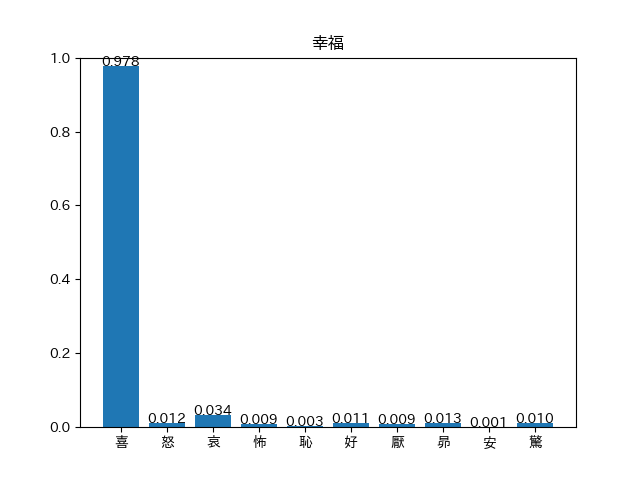
\includegraphics[keepaspectratio, scale=0.45]{./figure/BERT+weight/Q05/001.png}
			\subcaption{「幸福」に対する感情ベクトル}
		\end{minipage} &
		\begin{minipage}[t]{0.45\hsize}
			\centering
			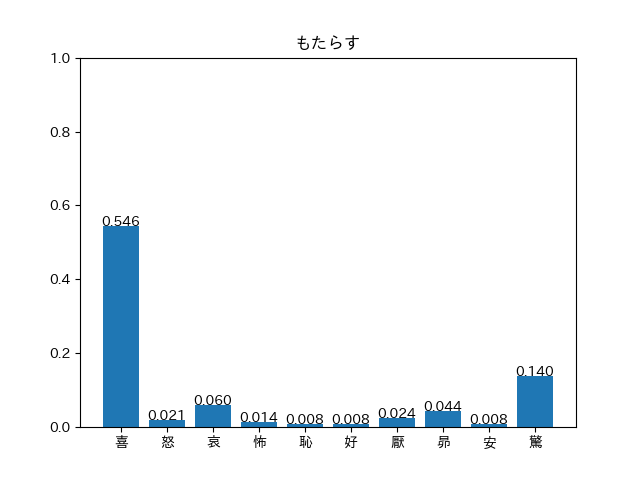
\includegraphics[keepaspectratio, scale=0.45]{./figure/BERT+weight/Q05/002.png}
			\subcaption{「もたらす」に対する感情ベクトル}
		\end{minipage} \\
		\begin{minipage}[t]{0.45\hsize}
			\centering
			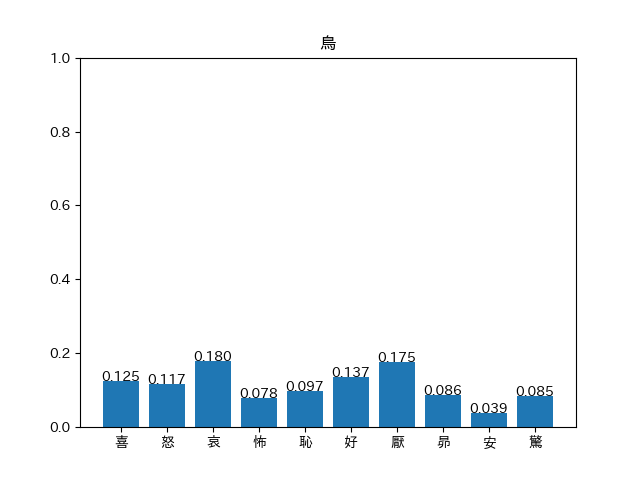
\includegraphics[keepaspectratio, scale=0.45]{./figure/BERT+weight/Q05/003.png}
			\subcaption{「鳥」に対する感情ベクトル}
		\end{minipage} \\
	\end{tabular}
	\caption{「幸福をもたらす鳥.」に対する各単語の感情ベクトル}
	\label{fig:output_q05}
\end{figure}

\begin{figure}[H]
	\begin{tabular}{cc}
		\begin{minipage}[t]{0.45\hsize}
			\centering
			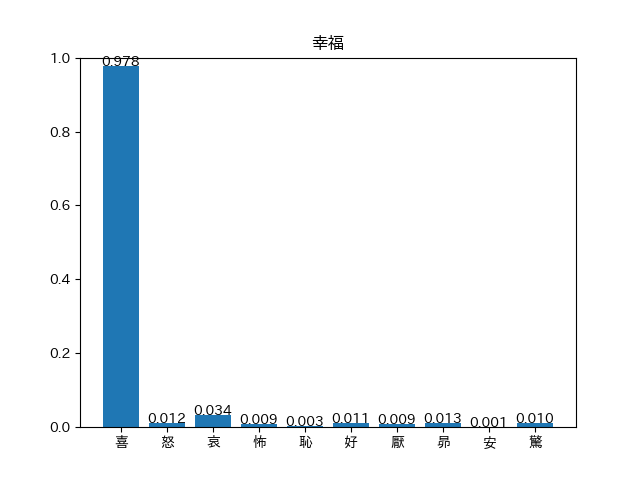
\includegraphics[keepaspectratio, scale=0.45]{./figure/BERT+weight/Q05/001.png}
			\subcaption{「不運」に対する感情ベクトル}
		\end{minipage} &
		\begin{minipage}[t]{0.45\hsize}
			\centering
			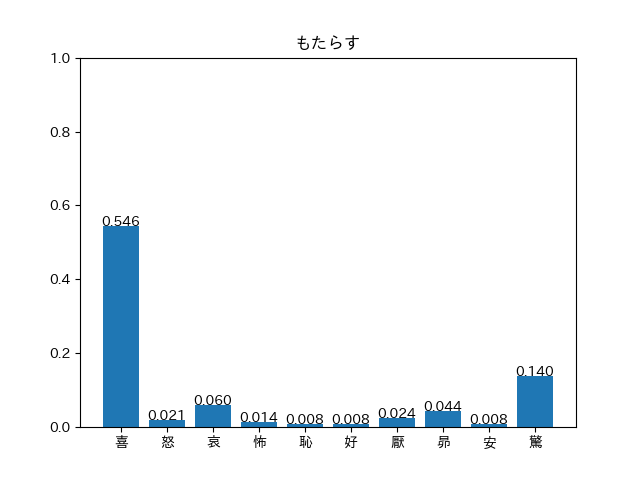
\includegraphics[keepaspectratio, scale=0.45]{./figure/BERT+weight/Q05/002.png}
			\subcaption{「もたらす」に対する感情ベクトル}
		\end{minipage} \\
		\begin{minipage}[t]{0.45\hsize}
			\centering
			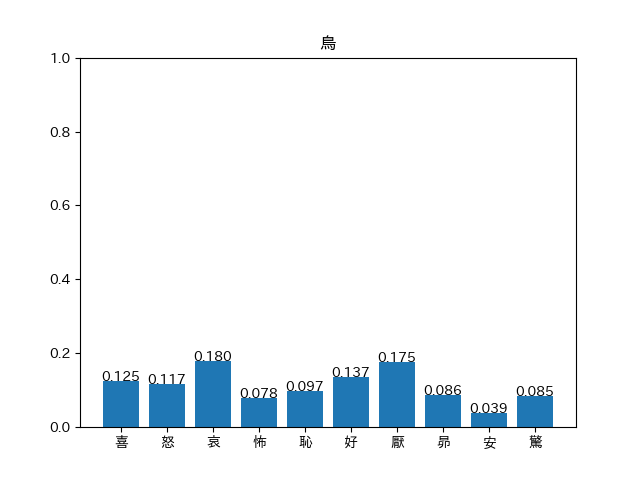
\includegraphics[keepaspectratio, scale=0.45]{./figure/BERT+weight/Q05/003.png}
			\subcaption{「行い」に対する感情ベクトル}
		\end{minipage} \\
	\end{tabular}
	\caption{「不運をもたらす行い.」に対する各単語の感情ベクトル}
	\label{fig:output_q06}
\end{figure}

\begin{figure}[H]
	\begin{tabular}{cc}
		\begin{minipage}[t]{0.45\hsize}
			\centering
			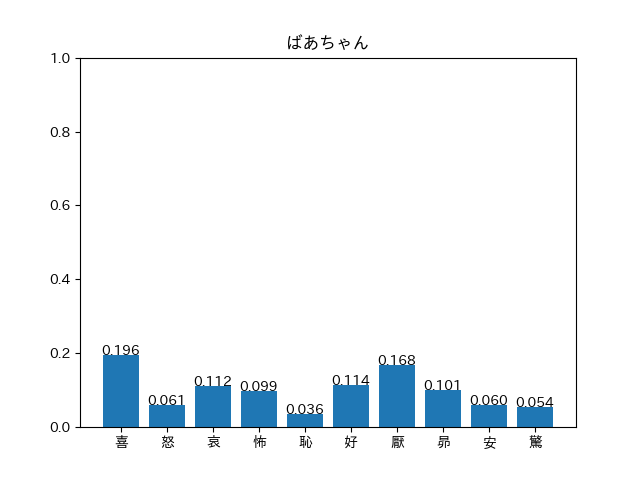
\includegraphics[keepaspectratio, scale=0.45]{./figure/BERT+weight/Q11/001.png}
			\subcaption{「ばあちゃん」に対する感情ベクトル}
		\end{minipage} &
		\begin{minipage}[t]{0.45\hsize}
			\centering
			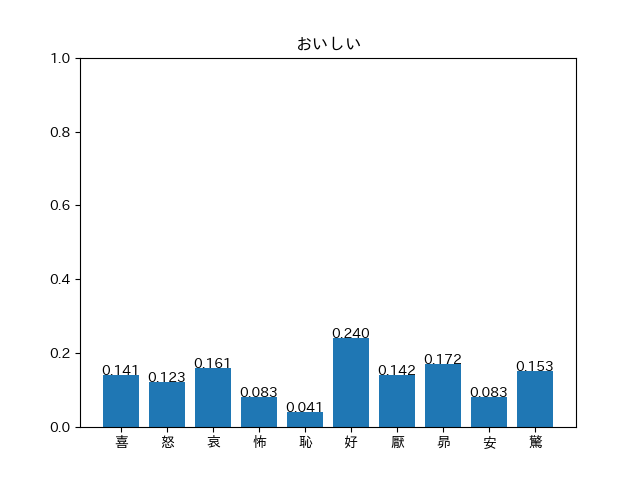
\includegraphics[keepaspectratio, scale=0.45]{./figure/BERT+weight/Q11/002.png}
			\subcaption{「おいしい」に対する感情ベクトル}
		\end{minipage} \\
		\begin{minipage}[t]{0.45\hsize}
			\centering
			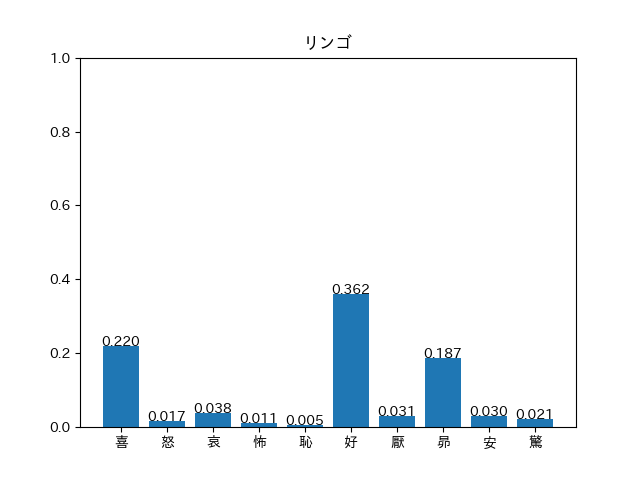
\includegraphics[keepaspectratio, scale=0.45]{./figure/BERT+weight/Q11/003.png}
			\subcaption{「リンゴ」に対する感情ベクトル}
		\end{minipage} &
		\begin{minipage}[t]{0.45\hsize}
			\centering
			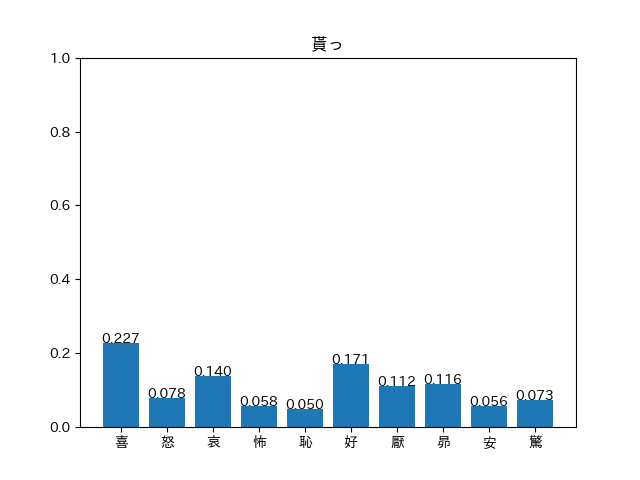
\includegraphics[keepaspectratio, scale=0.45]{./figure/BERT+weight/Q11/004.png}
			\subcaption{「貰っ」に対する感情ベクトル}
		\end{minipage} \\
	\end{tabular}
	\caption{「おばあちゃんからおいしいリンゴを貰った.」に対する各単語の感情ベクトル}
	\label{fig:output_q11}
\end{figure}

\begin{figure}[H]
	\begin{tabular}{cc}
		\begin{minipage}[t]{0.45\hsize}
			\centering
			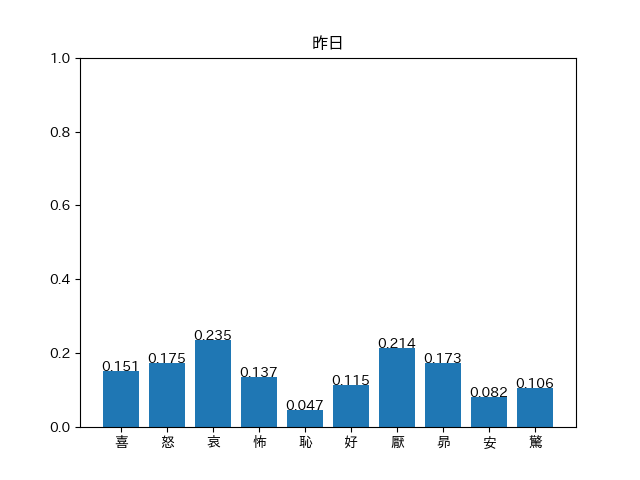
\includegraphics[keepaspectratio, scale=0.45]{./figure/BERT+weight/Q12/001.png}
			\subcaption{「昨日」に対する感情ベクトル}
		\end{minipage} &
		\begin{minipage}[t]{0.45\hsize}
			\centering
			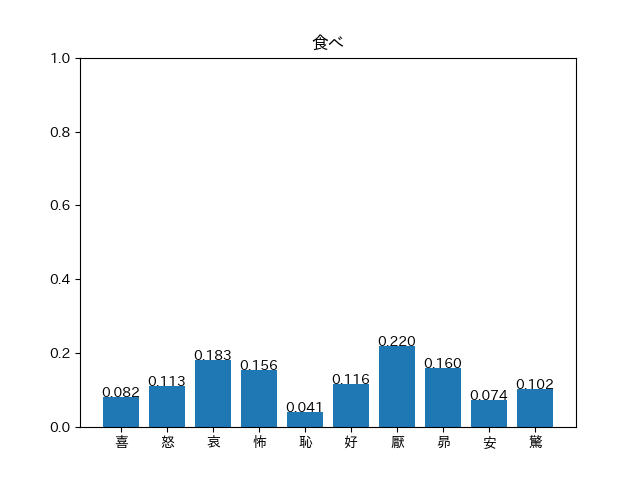
\includegraphics[keepaspectratio, scale=0.45]{./figure/BERT+weight/Q12/002.png}
			\subcaption{「食べ」に対する感情ベクトル}
		\end{minipage} \\
		\begin{minipage}[t]{0.45\hsize}
			\centering
			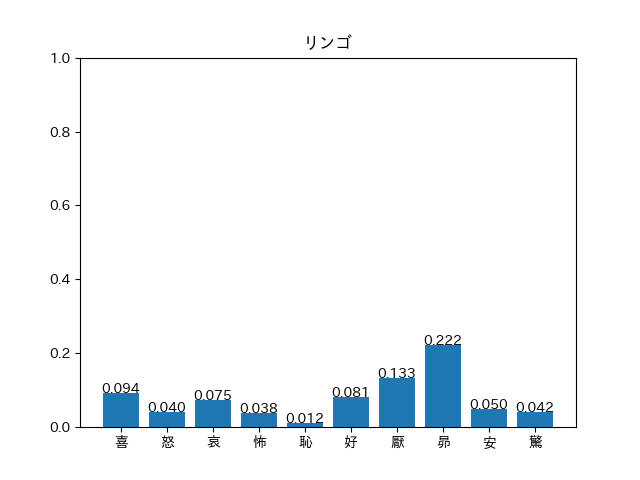
\includegraphics[keepaspectratio, scale=0.45]{./figure/BERT+weight/Q12/003.png}
			\subcaption{「リンゴ」に対する感情ベクトル}
		\end{minipage} &
		\begin{minipage}[t]{0.45\hsize}
			\centering
			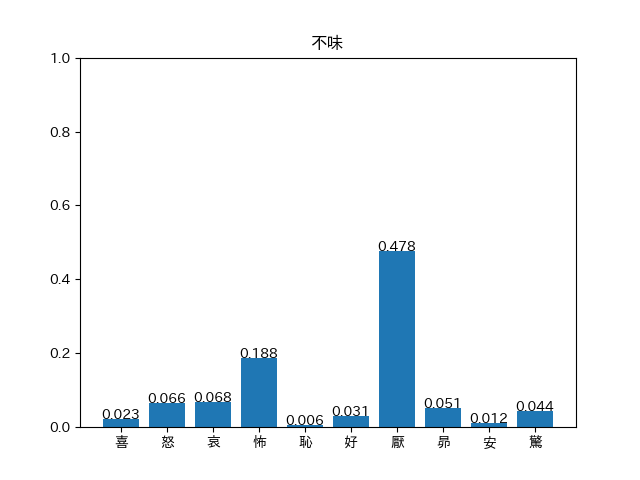
\includegraphics[keepaspectratio, scale=0.45]{./figure/BERT+weight/Q12/004.png}
			\subcaption{「不味」に対する感情ベクトル}
		\end{minipage} \\
	\end{tabular}
	\caption{「昨日食べたリンゴが不味すぎた.」に対する各単語の感情ベクトル}
	\label{fig:output_q12}
\end{figure}

\begin{figure}[H]
	\begin{tabular}{cc}
		\begin{minipage}[t]{0.45\hsize}
			\centering
			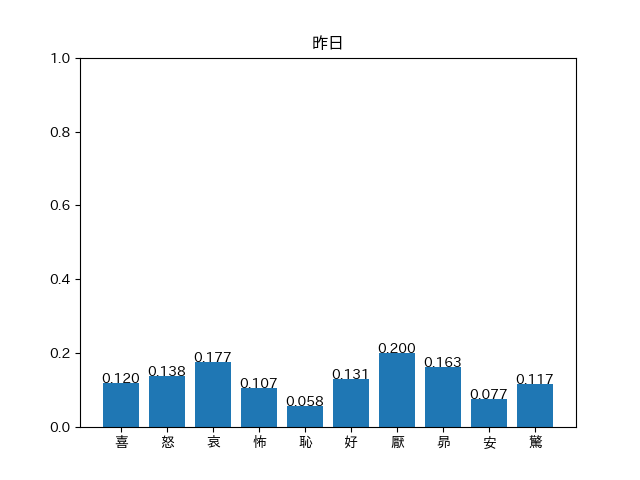
\includegraphics[keepaspectratio, scale=0.45]{./figure/BERT+weight/Q23/001.png}
			\subcaption{「昨日」に対する感情ベクトル}
		\end{minipage} &
		\begin{minipage}[t]{0.45\hsize}
			\centering
			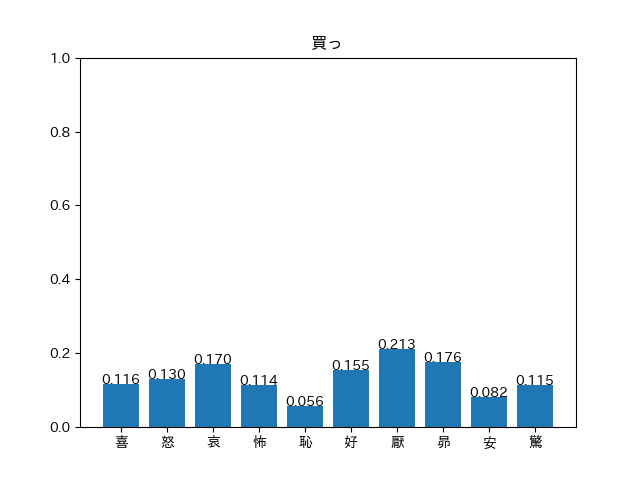
\includegraphics[keepaspectratio, scale=0.45]{./figure/BERT+weight/Q23/002.png}
			\subcaption{「買っ」に対する感情ベクトル}
		\end{minipage} \\
		\begin{minipage}[t]{0.45\hsize}
			\centering
			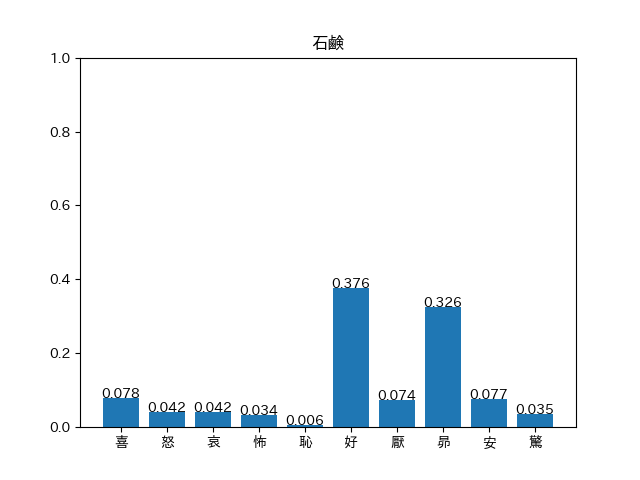
\includegraphics[keepaspectratio, scale=0.45]{./figure/BERT+weight/Q23/003.png}
			\subcaption{「石鹸」に対する感情ベクトル}
		\end{minipage} &
		\begin{minipage}[t]{0.45\hsize}
			\centering
			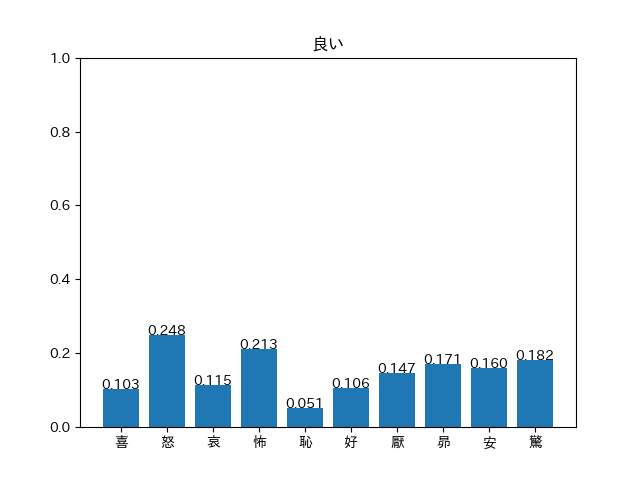
\includegraphics[keepaspectratio, scale=0.45]{./figure/BERT+weight/Q23/004.png}
			\subcaption{「良い」に対する感情ベクトル}
		\end{minipage} \\
		\begin{minipage}[t]{0.45\hsize}
			\centering
			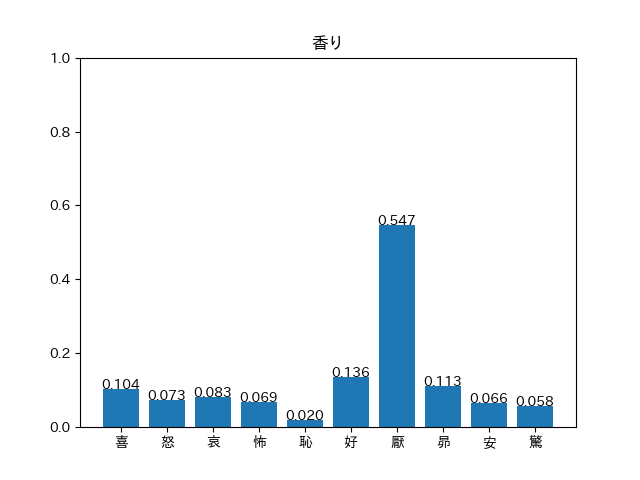
\includegraphics[keepaspectratio, scale=0.45]{./figure/BERT+weight/Q23/005.png}
			\subcaption{「香り」に対する感情ベクトル}
		\end{minipage} \\
	\end{tabular}
	\caption{「昨日買った石鹸は良い香りがする.」に対する各単語の感情ベクトル}
	\label{fig:output_q23}
\end{figure}

\begin{figure}[H]
	\begin{tabular}{cc}
		\begin{minipage}[t]{0.45\hsize}
			\centering
			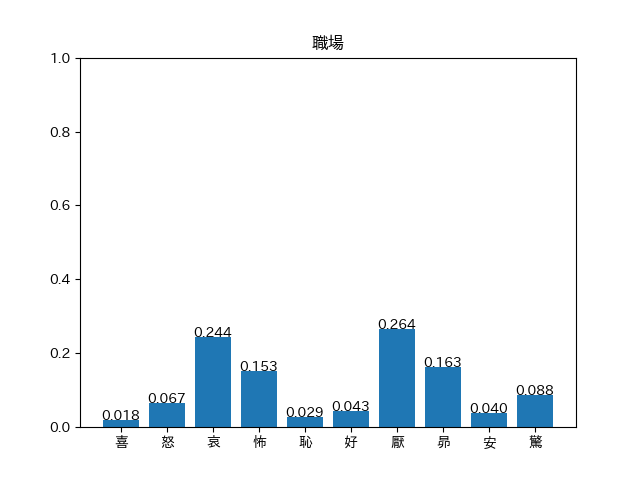
\includegraphics[keepaspectratio, scale=0.45]{./figure/BERT+weight/Q24/001.png}
			\subcaption{「職場」に対する感情ベクトル}
		\end{minipage} &
		\begin{minipage}[t]{0.45\hsize}
			\centering
			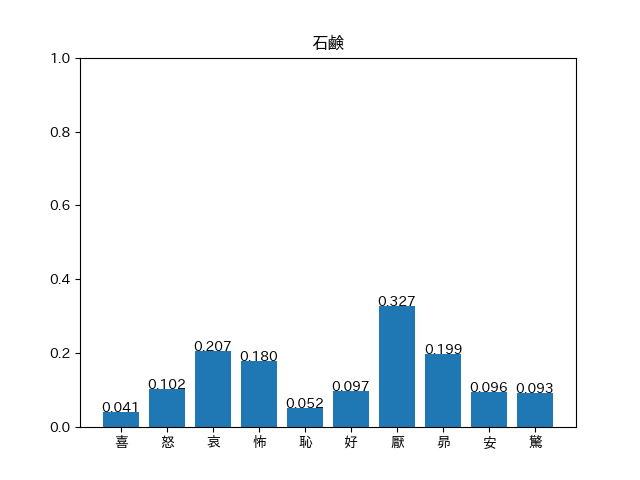
\includegraphics[keepaspectratio, scale=0.45]{./figure/BERT+weight/Q24/002.png}
			\subcaption{「石鹸」に対する感情ベクトル}
		\end{minipage} \\
		\begin{minipage}[t]{0.45\hsize}
			\centering
			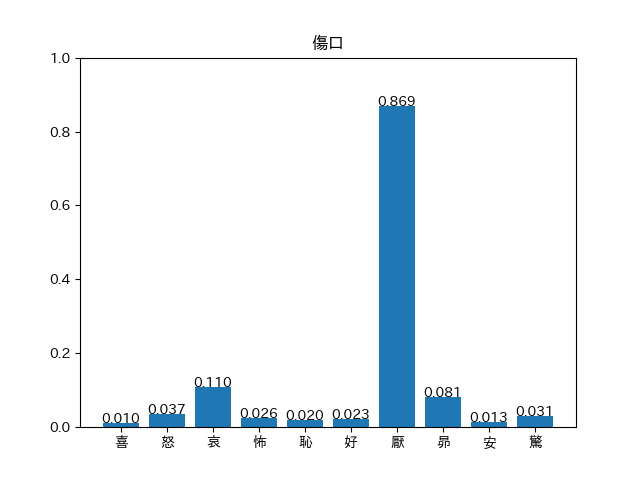
\includegraphics[keepaspectratio, scale=0.45]{./figure/BERT+weight/Q24/003.png}
			\subcaption{「傷口」に対する感情ベクトル}
		\end{minipage} \\
	\end{tabular}
	\caption{「職場の石鹸は傷口に沁みる.」に対する各単語の感情ベクトル}
	\label{fig:output_q24}
\end{figure}

\begin{figure}[H]
	\begin{tabular}{cc}
		\begin{minipage}[t]{0.45\hsize}
			\centering
			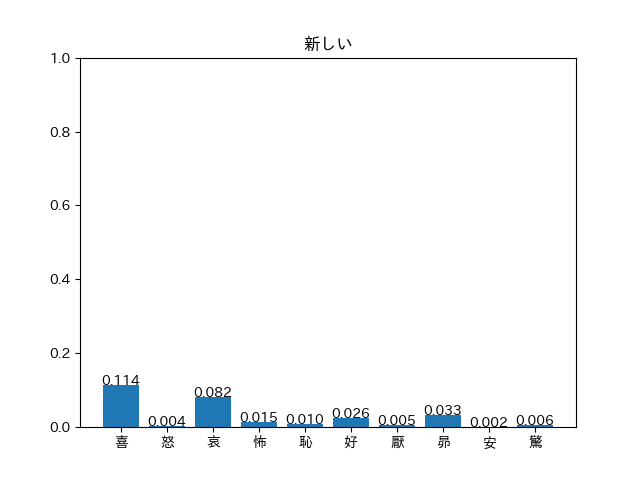
\includegraphics[keepaspectratio, scale=0.45]{./figure/BERT+weight/Q29/001.png}
			\subcaption{「新しい」に対する感情ベクトル}
		\end{minipage} &
		\begin{minipage}[t]{0.45\hsize}
			\centering
			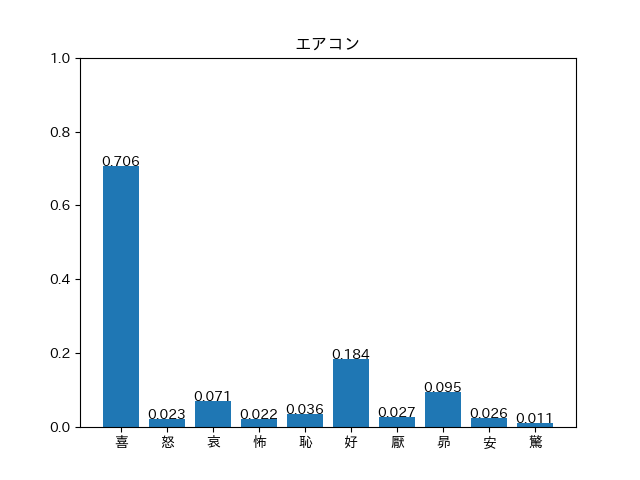
\includegraphics[keepaspectratio, scale=0.45]{./figure/BERT+weight/Q29/002.png}
			\subcaption{「エアコン」に対する感情ベクトル}
		\end{minipage} \\
		\begin{minipage}[t]{0.45\hsize}
			\centering
			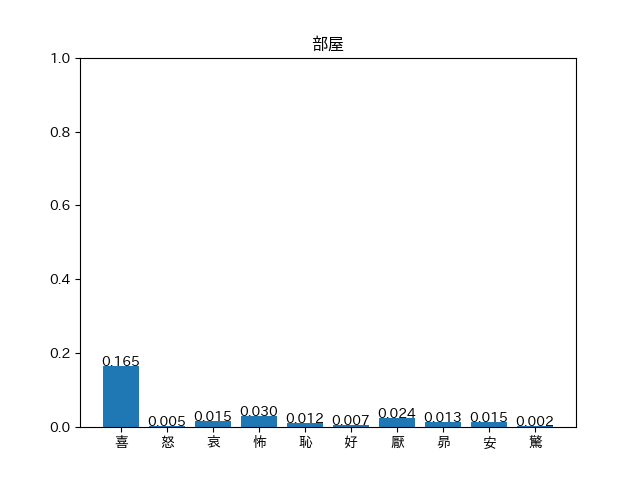
\includegraphics[keepaspectratio, scale=0.45]{./figure/BERT+weight/Q29/003.png}
			\subcaption{「部屋」に対する感情ベクトル}
		\end{minipage} &
		\begin{minipage}[t]{0.45\hsize}
			\centering
			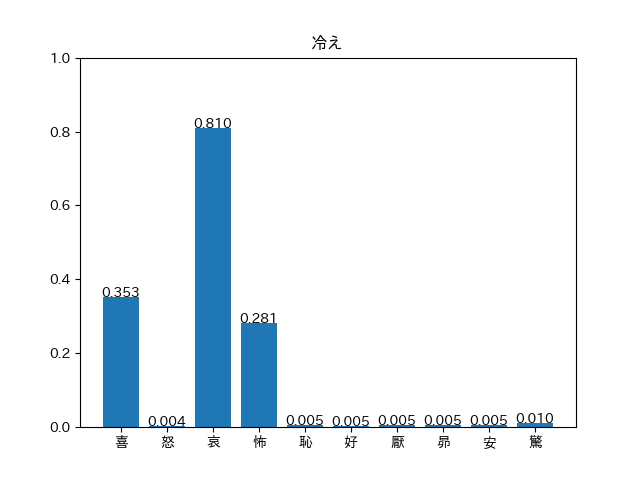
\includegraphics[keepaspectratio, scale=0.45]{./figure/BERT+weight/Q29/004.png}
			\subcaption{「冷え」に対する感情ベクトル}
		\end{minipage} \\
		\begin{minipage}[t]{0.45\hsize}
			\centering
			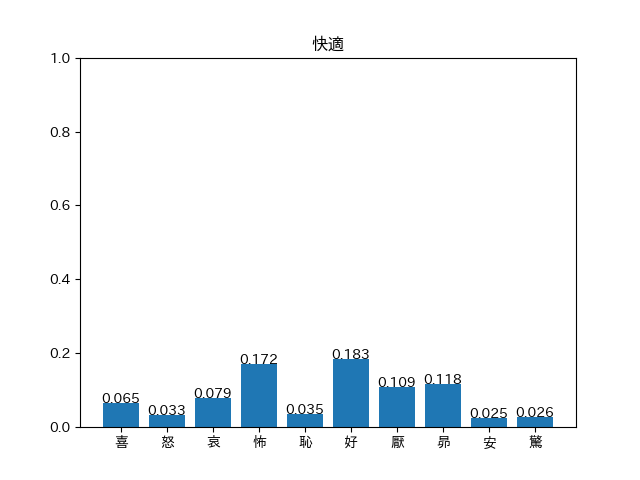
\includegraphics[keepaspectratio, scale=0.45]{./figure/BERT+weight/Q29/005.png}
			\subcaption{「快適」に対する感情ベクトル}
		\end{minipage} \\
	\end{tabular}
	\caption{「新しいエアコンは、部屋がよく冷えてとても快適である.」に対する各単語の感情ベクトル}
	\label{fig:output_q29}
\end{figure}

\begin{figure}[H]
	\begin{tabular}{cc}
		\begin{minipage}[t]{0.45\hsize}
			\centering
			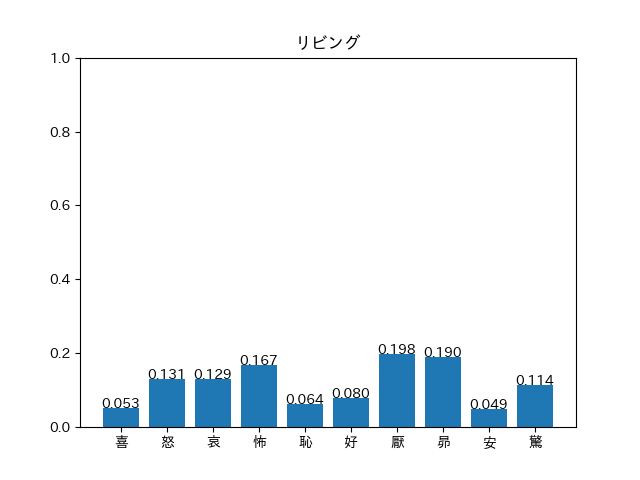
\includegraphics[keepaspectratio, scale=0.45]{./figure/BERT+weight/Q30/001.png}
			\subcaption{「リビング」に対する感情ベクトル}
		\end{minipage} &
		\begin{minipage}[t]{0.45\hsize}
			\centering
			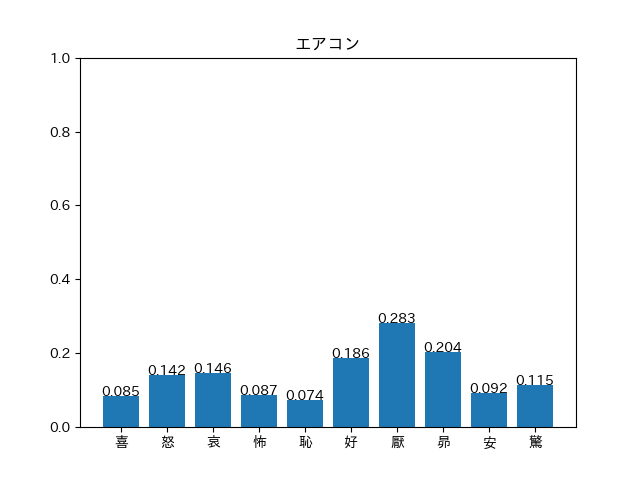
\includegraphics[keepaspectratio, scale=0.45]{./figure/BERT+weight/Q30/002.png}
			\subcaption{「エアコン」に対する感情ベクトル}
		\end{minipage} \\
		\begin{minipage}[t]{0.45\hsize}
			\centering
			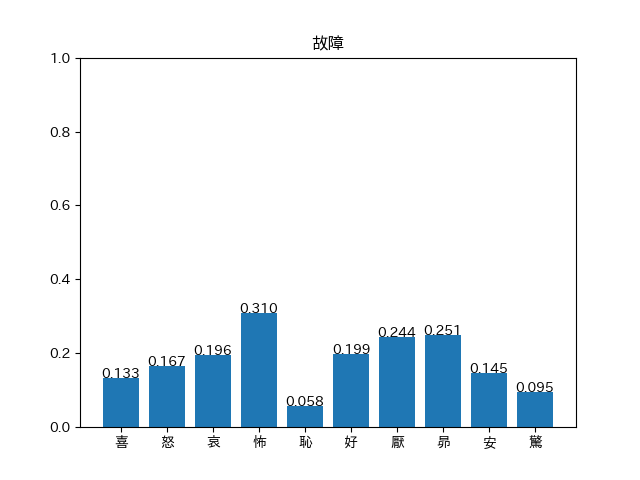
\includegraphics[keepaspectratio, scale=0.45]{./figure/BERT+weight/Q30/003.png}
			\subcaption{「故障」に対する感情ベクトル}
		\end{minipage} &
		\begin{minipage}[t]{0.45\hsize}
			\centering
			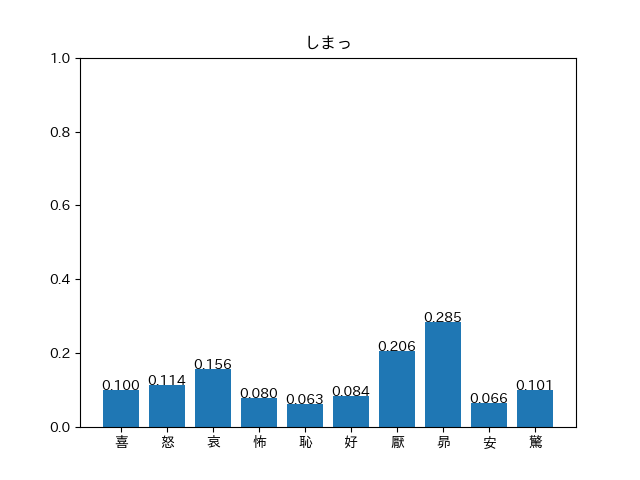
\includegraphics[keepaspectratio, scale=0.45]{./figure/BERT+weight/Q30/004.png}
			\subcaption{「しまっ」に対する感情ベクトル}
		\end{minipage} \\
	\end{tabular}
	\caption{「リビングのエアコンが故障してしまった.」に対する各単語の感情ベクトル}
	\label{fig:output_q30}
\end{figure}

\begin{figure}[H]
	\begin{tabular}{cc}
		\begin{minipage}[t]{0.45\hsize}
			\centering
			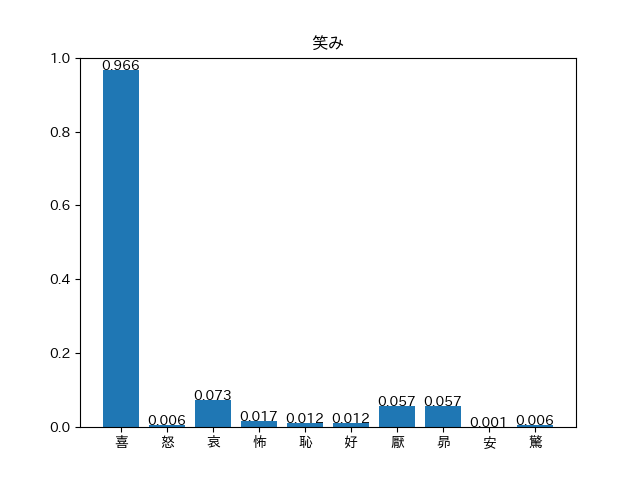
\includegraphics[keepaspectratio, scale=0.45]{./figure/BERT+weight/Q72/001.png}
			\subcaption{「笑み」に対する感情ベクトル}
		\end{minipage} &
		\begin{minipage}[t]{0.45\hsize}
			\centering
			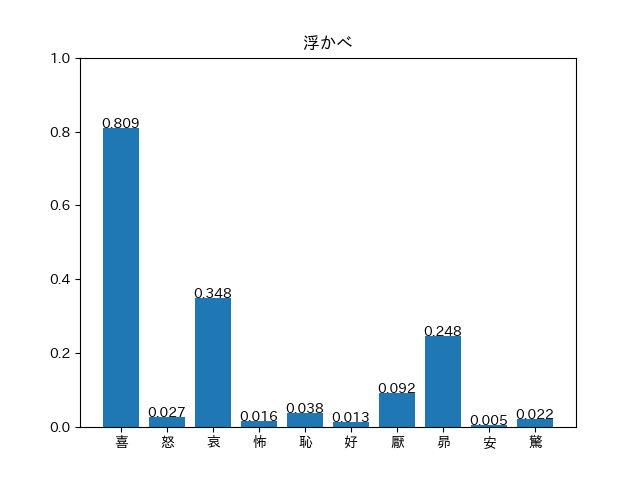
\includegraphics[keepaspectratio, scale=0.45]{./figure/BERT+weight/Q72/002.png}
			\subcaption{「浮かべ」に対する感情ベクトル}
		\end{minipage} \\
	\end{tabular}
	\caption{「彼は笑みを浮かべた.」に対する各単語の感情ベクトル}
	\label{fig:output_q72}
\end{figure}

\begin{figure}[H]
	\begin{tabular}{cc}
		\begin{minipage}[t]{0.45\hsize}
			\centering
			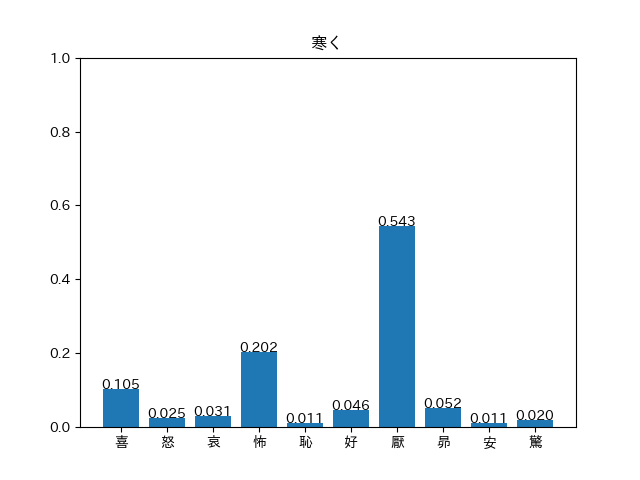
\includegraphics[keepaspectratio, scale=0.45]{./figure/BERT+weight/Q74/001.png}
			\subcaption{「寒く」に対する感情ベクトル}
		\end{minipage} &
		\begin{minipage}[t]{0.45\hsize}
			\centering
			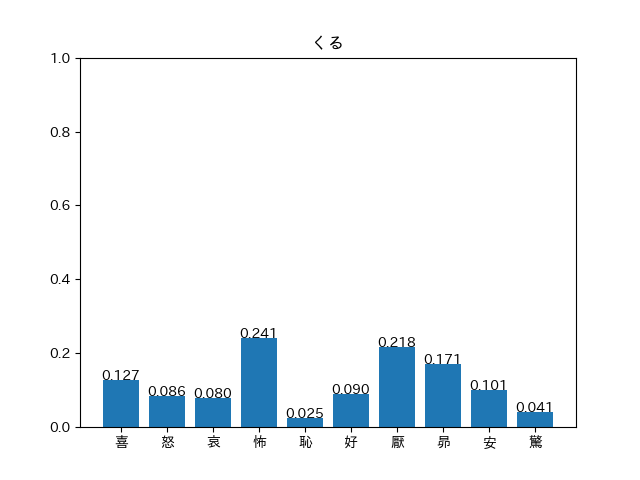
\includegraphics[keepaspectratio, scale=0.45]{./figure/BERT+weight/Q74/002.png}
			\subcaption{「くる」に対する感情ベクトル}
		\end{minipage} \\
		\begin{minipage}[t]{0.45\hsize}
			\centering
			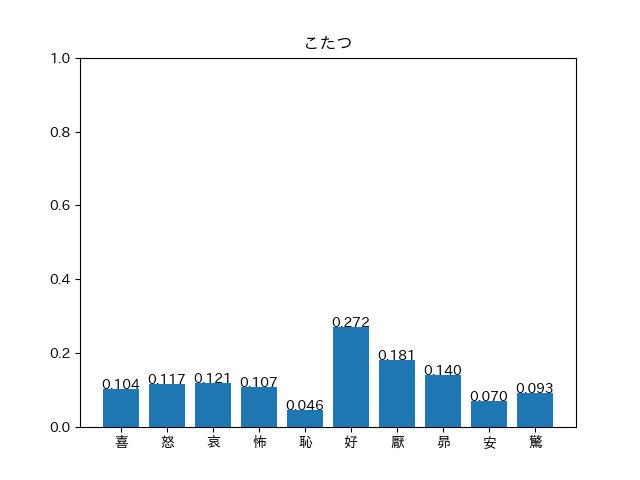
\includegraphics[keepaspectratio, scale=0.45]{./figure/BERT+weight/Q74/003.png}
			\subcaption{「こたつ」に対する感情ベクトル}
		\end{minipage} &
		\begin{minipage}[t]{0.45\hsize}
			\centering
			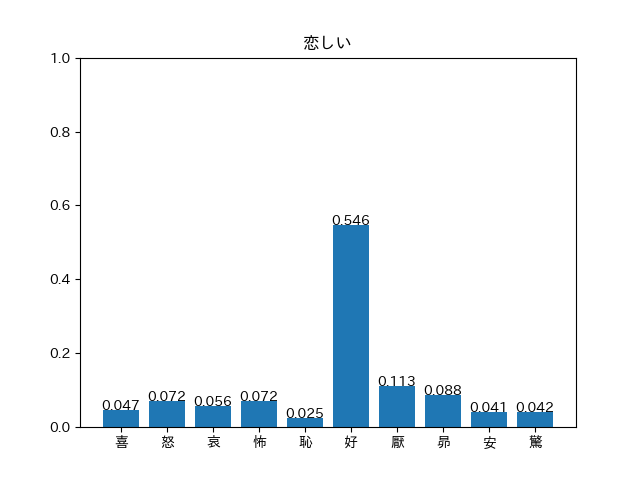
\includegraphics[keepaspectratio, scale=0.45]{./figure/BERT+weight/Q74/004.png}
			\subcaption{「恋しい」に対する感情ベクトル}
		\end{minipage} \\
	\end{tabular}
	\caption{「寒くなってくると、こたつが恋しい.」に対する各単語の感情ベクトル}
	\label{fig:output_q74}
\end{figure}

\begin{figure}[H]
	\begin{tabular}{cc}
		\begin{minipage}[t]{0.45\hsize}
			\centering
			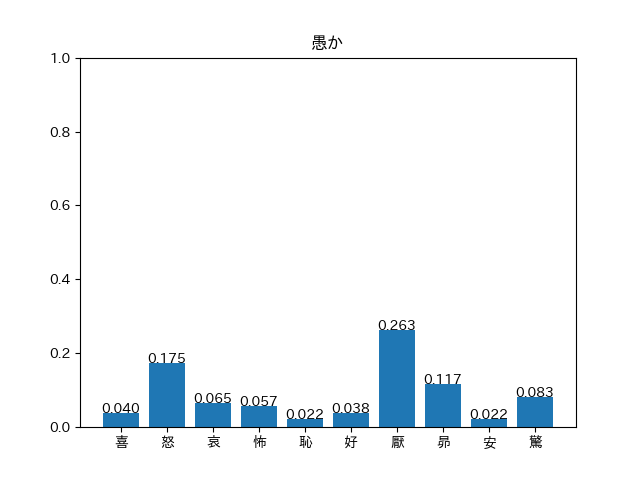
\includegraphics[keepaspectratio, scale=0.45]{./figure/BERT+weight/Q80/001.png}
			\subcaption{「愚か」に対する感情ベクトル}
		\end{minipage} &
		\begin{minipage}[t]{0.45\hsize}
			\centering
			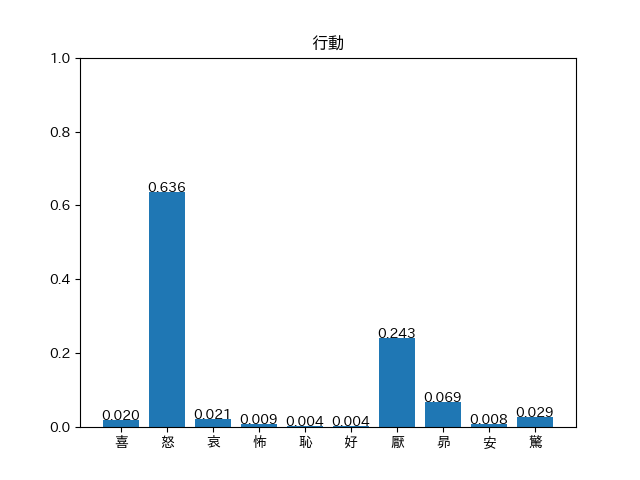
\includegraphics[keepaspectratio, scale=0.45]{./figure/BERT+weight/Q80/002.png}
			\subcaption{「行動」に対する感情ベクトル}
		\end{minipage} \\
		\begin{minipage}[t]{0.45\hsize}
			\centering
			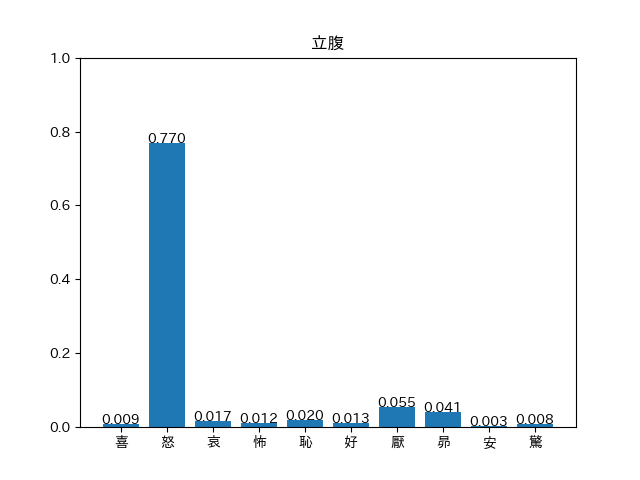
\includegraphics[keepaspectratio, scale=0.45]{./figure/BERT+weight/Q80/003.png}
			\subcaption{「立腹」に対する感情ベクトル}
		\end{minipage} \\
	\end{tabular}
	\caption{「愚かな行動に立腹した.」に対する各単語の感情ベクトル}
	\label{fig:output_q80}
\end{figure}

\begin{figure}[H]
	\begin{tabular}{cc}
		\begin{minipage}[t]{0.45\hsize}
			\centering
			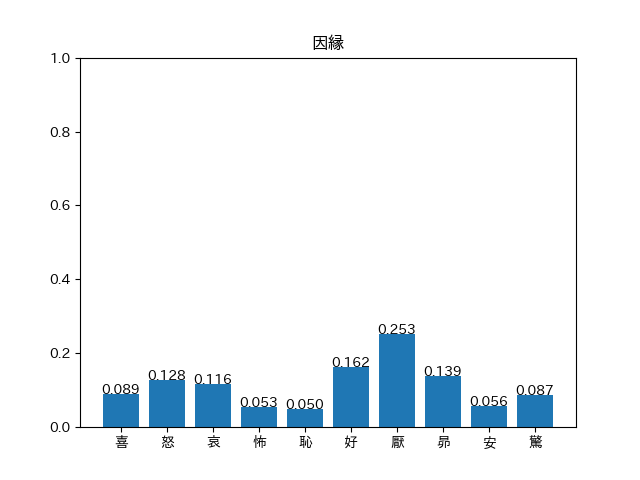
\includegraphics[keepaspectratio, scale=0.45]{./figure/BERT+weight/Q85/001.png}
			\subcaption{「因縁」に対する感情ベクトル}
		\end{minipage} &
		\begin{minipage}[t]{0.45\hsize}
			\centering
			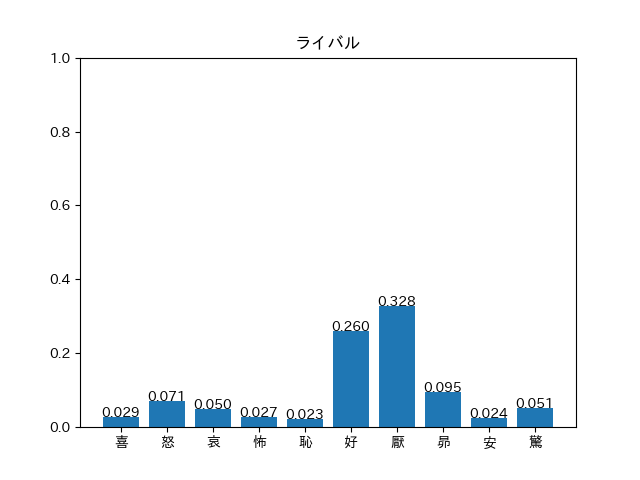
\includegraphics[keepaspectratio, scale=0.45]{./figure/BERT+weight/Q85/002.png}
			\subcaption{「ライバル」に対する感情ベクトル}
		\end{minipage} \\
		\begin{minipage}[t]{0.45\hsize}
			\centering
			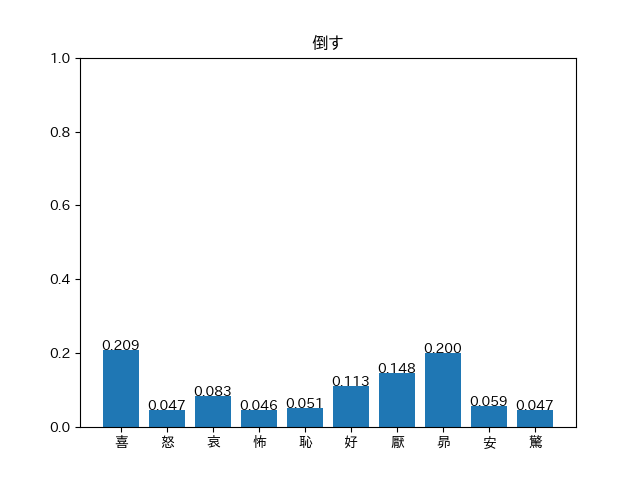
\includegraphics[keepaspectratio, scale=0.45]{./figure/BERT+weight/Q85/003.png}
			\subcaption{「倒す」に対する感情ベクトル}
		\end{minipage} &
		\begin{minipage}[t]{0.45\hsize}
			\centering
			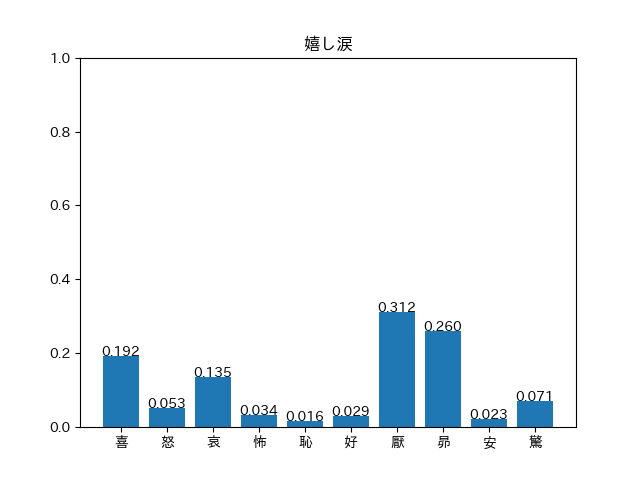
\includegraphics[keepaspectratio, scale=0.45]{./figure/BERT+weight/Q85/004.png}
			\subcaption{「嬉し涙」に対する感情ベクトル}
		\end{minipage} \\
		\begin{minipage}[t]{0.45\hsize}
			\centering
			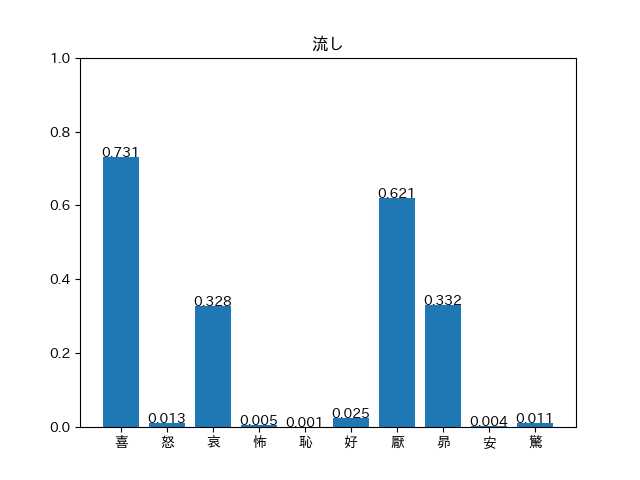
\includegraphics[keepaspectratio, scale=0.45]{./figure/BERT+weight/Q85/005.png}
			\subcaption{「流し」に対する感情ベクトル}
		\end{minipage} \\
	\end{tabular}
	\caption{「因縁のライバルを倒すことができ、嬉し涙を流した.」に対する各単語の感情ベクトル}
	\label{fig:output_q85}
\end{figure}

\begin{figure}[H]
	\begin{tabular}{cc}
		\begin{minipage}[t]{0.45\hsize}
			\centering
			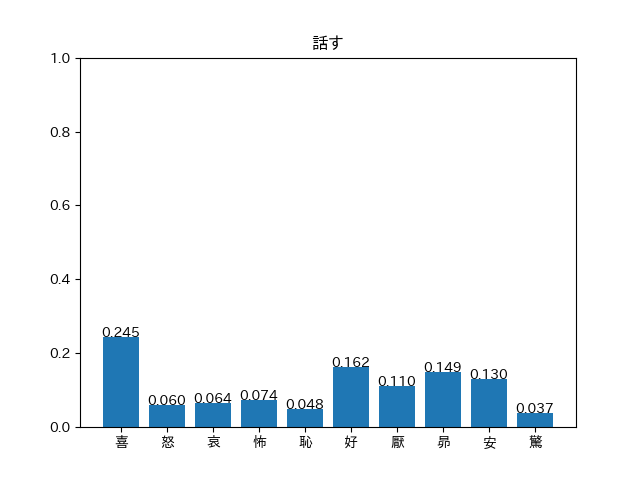
\includegraphics[keepaspectratio, scale=0.45]{./figure/BERT+weight/Q39/001.png}
			\subcaption{「話す」に対する感情ベクトル}
		\end{minipage} &
		\begin{minipage}[t]{0.45\hsize}
			\centering
			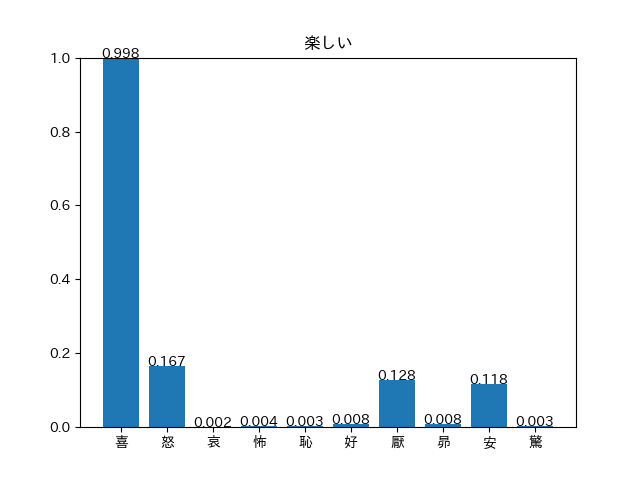
\includegraphics[keepaspectratio, scale=0.45]{./figure/BERT+weight/Q39/002.png}
			\subcaption{「楽しい」に対する感情ベクトル}
		\end{minipage} \\
		\begin{minipage}[t]{0.45\hsize}
			\centering
			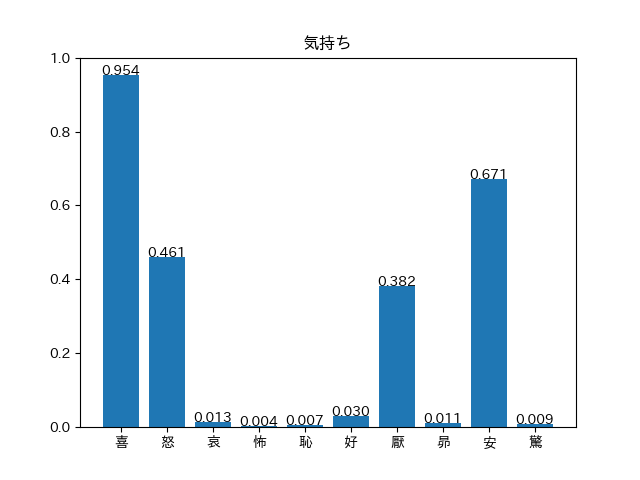
\includegraphics[keepaspectratio, scale=0.45]{./figure/BERT+weight/Q39/003.png}
			\subcaption{「気持ち」に対する感情ベクトル}
		\end{minipage} \\
	\end{tabular}
	\caption{「彼女と話すと楽しい気持ちになる.」に対する各単語の感情ベクトル}
	\label{fig:output_q39}
\end{figure}

\begin{figure}[H]
	\begin{tabular}{cc}
		\begin{minipage}[t]{0.45\hsize}
			\centering
			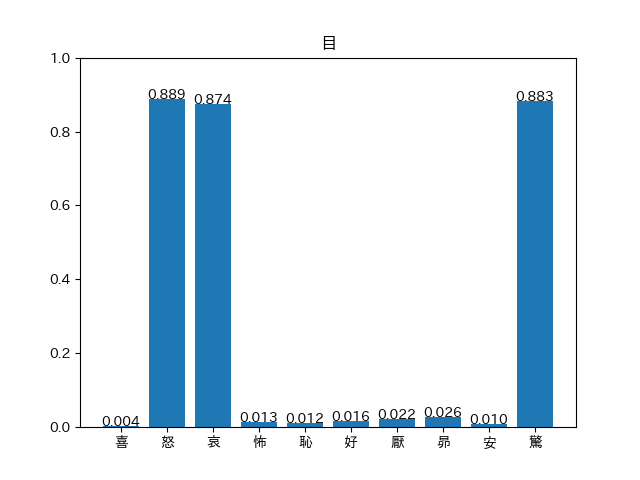
\includegraphics[keepaspectratio, scale=0.45]{./figure/BERT+weight/Q43/001.png}
			\subcaption{「目」に対する感情ベクトル}
		\end{minipage} &
		\begin{minipage}[t]{0.45\hsize}
			\centering
			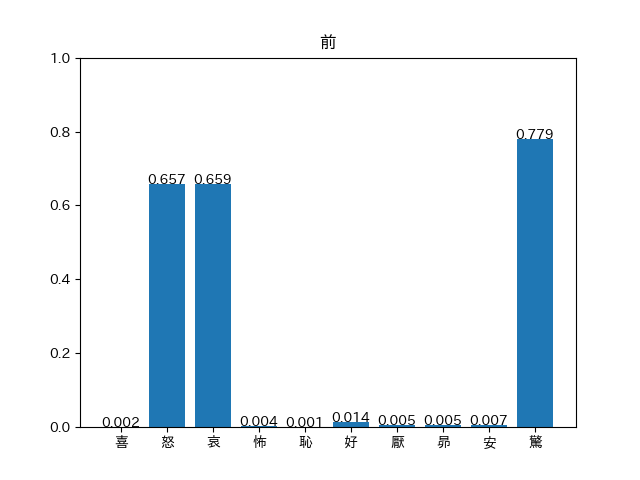
\includegraphics[keepaspectratio, scale=0.45]{./figure/BERT+weight/Q43/002.png}
			\subcaption{「前」に対する感情ベクトル}
		\end{minipage} \\
		\begin{minipage}[t]{0.45\hsize}
			\centering
			\includegraphics[keepaspectratio, scale=0.45]{./figure/BERT+weight/Q43/003.png}
			\subcaption{「事故」に対する感情ベクトル}
		\end{minipage} &
		\begin{minipage}[t]{0.45\hsize}
			\centering
			\includegraphics[keepaspectratio, scale=0.45]{./figure/BERT+weight/Q43/004.png}
			\subcaption{「見」に対する感情ベクトル}
		\end{minipage} \\
		\begin{minipage}[t]{0.45\hsize}
			\centering
			\includegraphics[keepaspectratio, scale=0.45]{./figure/BERT+weight/Q43/005.png}
			\subcaption{「悲しい」に対する感情ベクトル}
		\end{minipage} &
		\begin{minipage}[t]{0.45\hsize}
			\centering
			\includegraphics[keepaspectratio, scale=0.45]{./figure/BERT+weight/Q43/006.png}
			\subcaption{「気持ち」に対する感情ベクトル}
		\end{minipage} \\
	\end{tabular}
	\caption{「目の前で大きな事故を見てしまい、悲しい気持ちになった.」に対する各単語の感情ベクトル}
	\label{fig:output_q43}
\end{figure}


\begin{figure}[H]
	\begin{tabular}{cc}
		\begin{minipage}[t]{0.45\hsize}
			\centering
			\includegraphics[keepaspectratio, scale=0.45]{./figure/BERT+weight/Q51/001.png}
			\subcaption{「久々」に対する感情ベクトル}
		\end{minipage} &
		\begin{minipage}[t]{0.45\hsize}
			\centering
			\includegraphics[keepaspectratio, scale=0.45]{./figure/BERT+weight/Q51/002.png}
			\subcaption{「再会」に対する感情ベクトル}
		\end{minipage} \\
		\begin{minipage}[t]{0.45\hsize}
			\centering
			\includegraphics[keepaspectratio, scale=0.45]{./figure/BERT+weight/Q51/003.png}
			\subcaption{「涙」に対する感情ベクトル}
		\end{minipage} &
		\begin{minipage}[t]{0.45\hsize}
			\centering
			\includegraphics[keepaspectratio, scale=0.45]{./figure/BERT+weight/Q51/004.png}
			\subcaption{「流し」に対する感情ベクトル}
		\end{minipage} \\
		\begin{minipage}[t]{0.45\hsize}
			\centering
			\includegraphics[keepaspectratio, scale=0.45]{./figure/BERT+weight/Q51/005.png}
			\subcaption{「喜ん」に対する感情ベクトル}
		\end{minipage} \\
	\end{tabular}
	\caption{「久々の再会に涙を流して喜んだ.」に対する各単語の感情ベクトル}
	\label{fig:output_q51}
\end{figure}

\begin{figure}[H]
	\begin{tabular}{cc}
		\begin{minipage}[t]{0.45\hsize}
			\centering
			\includegraphics[keepaspectratio, scale=0.45]{./figure/BERT+weight/Q55/001.png}
			\subcaption{「紛争」に対する感情ベクトル}
		\end{minipage} &
		\begin{minipage}[t]{0.45\hsize}
			\centering
			\includegraphics[keepaspectratio, scale=0.45]{./figure/BERT+weight/Q55/002.png}
			\subcaption{「悲惨」に対する感情ベクトル}
		\end{minipage} \\
		\begin{minipage}[t]{0.45\hsize}
			\centering
			\includegraphics[keepaspectratio, scale=0.45]{./figure/BERT+weight/Q55/003.png}
			\subcaption{「実態」に対する感情ベクトル}
		\end{minipage} &
		\begin{minipage}[t]{0.45\hsize}
			\centering
			\includegraphics[keepaspectratio, scale=0.45]{./figure/BERT+weight/Q55/004.png}
			\subcaption{「知り」に対する感情ベクトル}
		\end{minipage} \\
		\begin{minipage}[t]{0.45\hsize}
			\centering
			\includegraphics[keepaspectratio, scale=0.45]{./figure/BERT+weight/Q55/005.png}
			\subcaption{「涙」に対する感情ベクトル}
		\end{minipage} &
		\begin{minipage}[t]{0.45\hsize}
			\centering
			\includegraphics[keepaspectratio, scale=0.45]{./figure/BERT+weight/Q55/006.png}
			\subcaption{「止まら」に対する感情ベクトル}
		\end{minipage} \\
	\end{tabular}
	\caption{「紛争の悲惨な実態を知り、涙が止まらない.」に対する各単語の感情ベクトル}
	\label{fig:output_q55}
\end{figure}

\begin{figure}[H]
	\begin{tabular}{cc}
		\begin{minipage}[t]{0.45\hsize}
			\centering
			\includegraphics[keepaspectratio, scale=0.45]{./figure/BERT+weight/Q62/001.png}
			\subcaption{「世界一」に対する感情ベクトル}
		\end{minipage} &
		\begin{minipage}[t]{0.45\hsize}
			\centering
			\includegraphics[keepaspectratio, scale=0.45]{./figure/BERT+weight/Q62/002.png}
			\subcaption{「選手」に対する感情ベクトル}
		\end{minipage} \\
		\begin{minipage}[t]{0.45\hsize}
			\centering
			\includegraphics[keepaspectratio, scale=0.45]{./figure/BERT+weight/Q62/003.png}
			\subcaption{「たい」に対する感情ベクトル}
		\end{minipage} &
		\begin{minipage}[t]{0.45\hsize}
			\centering
			\includegraphics[keepaspectratio, scale=0.45]{./figure/BERT+weight/Q62/004.png}
			\subcaption{「思い」に対する感情ベクトル}
		\end{minipage} \\
		\begin{minipage}[t]{0.45\hsize}
			\centering
			\includegraphics[keepaspectratio, scale=0.45]{./figure/BERT+weight/Q62/005.png}
			\subcaption{「持っ」に対する感情ベクトル}
		\end{minipage} \\
	\end{tabular}
	\caption{「彼は世界一の選手になりたいという思いを持っている.」に対する各単語の感情ベクトル}
	\label{fig:output_q62}
\end{figure}

\begin{figure}[H]
	\begin{tabular}{cc}
		\begin{minipage}[t]{0.45\hsize}
			\centering
			\includegraphics[keepaspectratio, scale=0.45]{./figure/BERT+weight/Q69/001.png}
			\subcaption{「うまく」に対する感情ベクトル}
		\end{minipage} &
		\begin{minipage}[t]{0.45\hsize}
			\centering
			\includegraphics[keepaspectratio, scale=0.45]{./figure/BERT+weight/Q69/002.png}
			\subcaption{「多く」に対する感情ベクトル}
		\end{minipage} \\
		\begin{minipage}[t]{0.45\hsize}
			\centering
			\includegraphics[keepaspectratio, scale=0.45]{./figure/BERT+weight/Q69/003.png}
			\subcaption{「つらい」に対する感情ベクトル}
		\end{minipage} &
		\begin{minipage}[t]{0.45\hsize}
			\centering
			\includegraphics[keepaspectratio, scale=0.45]{./figure/BERT+weight/Q69/004.png}
			\subcaption{「思い」に対する感情ベクトル}
		\end{minipage} \\
		\begin{minipage}[t]{0.45\hsize}
			\centering
			\includegraphics[keepaspectratio, scale=0.45]{./figure/BERT+weight/Q69/005.png}
			\subcaption{「抱え」に対する感情ベクトル}
		\end{minipage} \\
	\end{tabular}
	\caption{「うまくいかないことが多く、つらい思いを抱えている.」に対する各単語の感情ベクトル}
	\label{fig:output_q69}
\end{figure}